\chapter{The Compost Bomb and the Terrestrial Carbon Cycle}
\label{chapter:global_bomb}
\graphicspath{{global_bomb/figs/}}

\todo[inline]{This is basically just going to be equations for now}


In \cref{chapter:continuous_compost_bomb} we saw how introducing a vertical dimension can affect the compost bomb.
We can also introduce horizontal dimensions into the problem. We therefore need to decide at what horizontal scale we
should work. We will work at the global-averaged scale motivated by work \parencite{Cox2006} which suggests a instability in the global
carbon cycle in certain parameter regimes. How does biogeochemical feedback affect this instability?

Following \cite{Luke2011}, we have the compost bomb equations
\begin{subequations}
  \label{eq:compost_bomb_equations}
  \begin{align}
    \mu \dv{T_s}{t} &= - \kappa \left(T_s - T_a\right) + Ar_0C_se^{\alpha T_s} \label{eq:compost_bomb_soil_temperature} \\
    \dv{C_s}{t} &= \Pi - r_0C_se^{\alpha T_s} \label{eq:compost_bomb_soil_carbon}
  \end{align}
\end{subequations}

Noting the obvious timescale seperation in \cref{eq:compost_bomb_equations} we can put \cref{eq:compost_bomb_soil_temperature} into
equilibrium to get
\begin{equation*}
  0 = - \kappa \left(T_s - T_a\right) + Ar_0C_se^{\alpha T_s}
\end{equation*}
which can be solved for the soil temperature to  give
\begin{equation}
  \label{eq:soil_temperature_equilibrium}
  T_s = T_a - \frac{1}{\alpha} W\left(-\frac{Ar_0C_s \alpha e^{\alpha T_a}}{\kappa} \right),
\end{equation}
where $W(x)$ is the Lambert $W$ function. The Lambert $W$ function, plotted in \cref{fig:lambert_W}, is defined as the solution to the equation
\begin{equation}
  \label{eq:lambert_W}
  W(x)e^{W(x)} = x.
\end{equation}

\begin{figure}
  \centering
  \begin{tikzpicture}
    \begin{axis}[
      xmin=-1,
      xmax=4,
      enlarge y limits=false,
      axis lines=left,
      xlabel=$x$,
      ylabel=$W(x)$,
      samples=50]
      \addplot[domain=-5:-1] (x * exp(x), x);
      \addplot[domain=-1:2] (x * exp(x), x);
    \end{axis}
  \end{tikzpicture}
  \caption{The Lambert $W$ function}
  \label{fig:lambert_W}
\end{figure}

Defining
\begin{equation}
  \label{eq:critical_npp}
  \Pi_c = \frac{\kappa}{\alpha A}
\end{equation}
we can rewrite \cref{eq:soil_temperature_equilibrium} as
\begin{equation}
  \label{eq:soil_temperature_equilibrium_nppc}
  T_s = T_a - \frac{1}{\alpha} W\left(-\frac{r_0C_s e^{\alpha T_a}}{\Pi_c} \right).
\end{equation}
We should therefore insert \cref{eq:soil_temperature_equilibrium_nppc} in \cref{eq:compost_bomb_soil_carbon}
to give
\begin{equation}
  \label{eq:soil_carbon_evolution}
  \dv{C_s}{t} = \Pi + \Pi_c W\left(-\frac{r_0C_s e^{\alpha T_a}}{\Pi_c} \right).
\end{equation}
This implies the equilibrium value of $C_s$ is
\begin{equation}
  \label{eq:equilibirum_soil_carbon}
  C_s^{\mathrm{eq}} = \frac{\Pi}{r_0} e^{-\alpha T_a} e^{-\Pi/\Pi_c}.
\end{equation}
Note that we recover the no biogeochemcial heating case by sending $\Pi_c \rightarrow \infty$.


Recognising that
\begin{equation}
  \label{eq:atmospheric_temperatures}
  T_a = \frac{S}{\log 2} \log \frac{C_a}{C_{a0}} 
\end{equation}
leads, upon substituting \cref{eq:atmospheric_temperatures} into \cref{eq:soil_carbon_evolution},
\begin{equation}
  \label{eq:global_soil_carbon}
  \dv{C_s}{t} = \Pi + \Pi_c W\left(-\frac{r_0C_s}{\Pi_c} \left(\frac{C_a}{C_{a0}}\right)^\mu \right),
\end{equation}
where
\begin{equation}
  \label{eq:mu}
  \mu = \frac{\alpha S}{\log 2}.
\end{equation}


We chose the temperature anomaly so that $T_a = 0$ corresponds to an equilibrium. We can then set
$r_0 = \frac{\Pi_0}{C_s^{\mathrm{eq}}}e^{-\Pi_0/\Pi_c}$, where $\Pi_0 = \Pi\left(C_{a0}\right)$.

To
numerically compute the equilibria of \cref{eq:global_soil_carbon} we need to define the dependence of $\Pi$ on
$C_a$  and the dependence of $C_a$ on $C_s$. We set NPP to
\begin{equation}
  \label{eq:npp_fertilization}
  \Pi(C_a) = \frac{\Pi_{\infty} C_a}{C_a + C_{a_{1/2}}}.
\end{equation}
This is an increasing function of $C_a$, which saturates to $\Pi_{\infty}$ for $C_a \gg C_{a_{1/2}}$.
We will assume  that a fixed fraction $\chi_0$ of atmospheric emissions reaches the ocean, meaning
\begin{equation}
  \label{eq:simple_ocean}
  C_a = C_{a0} -\frac{1}{1+\chi_0} (C_s - C_{s}^{\mathrm{eq}}).
  %C_s = C_{s}^{\mathrm{eq}} - (1 + \chi_0)(C_a - C_{a0}.
\end{equation}
It is now straightforward to compute the bifurcation diagram, which we do in \todo{bifurcation diagram!} 
\missingfigure{Bifurcation Diagram of \cref{eq:global_soil_carbon}}

We can make analytic progress too. To find the bifurcation we therefore just have to calculate where
\begin{equation*}
  \dv{\dot{C_s}}{C_s} = 0,
\end{equation*}
we will make use of
\begin{equation}
  \label{eq:derivative_of_lambert_W}
  W'(x) = \frac{W(x)}{x\left(1 + W\left(x\right)\right)}.
\end{equation}




Taking a derivative of the right hand side of \cref{eq:global_soil_carbon} and setting it to zero in equilibrium gives
\begin{equation}
  \label{eq:soil_carbon_lambda}
  \dv{\Pi}{C_a}\dv{C_a}{C_s} + \frac{\Pi_c}{C_s^{\mathrm{eq}}} \frac{W\left(-\frac{r_0C_s^{\mathrm{eq}}}{\Pi_c}\right)}{1+W\left(-\frac{r_0C_s^{\mathrm{eq}}}{\Pi_c}\right)} \left(
    1 + \mu \frac{C_s^{\mathrm{eq}}}{C_{a0}} \dv{C_a}{C_s}\right) = 0
\end{equation}
so
\begin{equation}
  \label{eq:critical_mu}
  \mu = -\frac{C_{a0}}{C_{s}^{\mathrm{eq}}}\dv{C_s}{C_a}\left(\dv{\Pi}{C_a}\dv{C_a}{C_s} \frac{C_s^{\mathrm{eq}}}{\Pi_c}\frac{1+W\left(-\frac{r_0C_s^{\mathrm{eq}}}{\Pi_c}\right)}{W\left(-\frac{r_0C_s^{\mathrm{eq}}}{\Pi_c}\right)} + 1 \right)
\end{equation}
which simplifies to
\begin{equation}
  \label{eq:critical_mu_simple_ocean}
  \mu = \left(1+\chi_0\right) \frac{C_{a0}}{C_{s}^{\mathrm{eq}}} -
  \frac{C_{a0}}{\Pi_c}\frac{1+W\left(-\frac{r_0C_s^{\mathrm{eq}}}{\Pi_c}\right)}{W\left(-\frac{r_0C_s^{\mathrm{eq}}}{\Pi_c}\right)}\dv{\Pi}{C_a}.
\end{equation}
This can be further reduced to
\begin{equation*}
  \mu = \left(1+\chi_0\right) \frac{C_{a0}}{C_{s}^{\mathrm{eq}}} -
  \frac{C_{a0}}{\Pi_c}
  \frac{1+W\left(-\frac{\Pi_0}{\Pi_c}\exp\left(-\frac{\Pi_0}{\Pi_c}\right)\right)}
  {W\left(-\frac{\Pi_0}{\Pi_c}\exp\left(-\frac{\Pi_0}{\Pi_c}\right)\right)}\dv{\Pi}{C_a} 
\end{equation*}
and even more to give
\begin{equation*}
  \mu = \left(1+\chi_0\right) \frac{C_{a0}}{C_{s}^{\mathrm{eq}}} -
  \frac{C_{a0}}{\Pi_c}
  \frac{1-\frac{\Pi_0}{\Pi_c}}{-\frac{\Pi_0}{\Pi_c}}\dv{\Pi}{C_a}.
\end{equation*}
Cleaning this up gives the final form.
\begin{equation}
  \label{eq:critical_mu_simple_ocean_in_terms_of_npp}
  \mu^* = \left(1+\chi_0\right) \frac{C_{a0}}{C_{s}^{\mathrm{eq}}} +
  \frac{C_{a0}}{\Pi_0} \dv{\Pi}{C_a} - \frac{C_{a0}}{\Pi_c}\dv{\Pi}{C_a}.
\end{equation}
We remark that taking the limit where $\Pi_c \rightarrow \infty$ gives
\begin{equation}
  \label{eq:mu_infinity}
  \mu^*_{\infty} =\left(1+\chi_0\right) \frac{C_{a0}}{C_{s}^{\mathrm{eq}}} +
  \frac{C_{a0}}{\Pi_0} \dv{\Pi}{C_a}.
\end{equation}
This corresponds to the limit where biogeochemcial heating does not occur.

% We note this implies a minimum allowed \ce{CO2} fertilization effect for a given $\mu$ (as we need $\mu < \mu_\infty^*$)
% \begin{equation}
%   \label{eq:minimum_allowed_co2_fertilization}
%   \dv{\Pi}{C_a} > \frac{\Pi_0\mu}{C_{a0}} - \frac{1+\chi_0}{C_s^{\mathrm{eq}}}\Pi_0
% \end{equation}


We can plot \cref{eq:critical_mu} to devide the parameter plane into a stable and unstable region.

\begin{figure}
  \centering
  \begin{tikzpicture}[
    /pgf/declare function={
      chi0 = 0.25;
      npp = 55.0;
      Ca0 = 589.0;
      Cseq = 1500.0;
    }
    ]
    \begin{axis}[
      legend pos=outer north east,
      % enlargelimits=false
      xlabel={$\Pi_c$},
      ylabel={$\mu$},
      xmin=20,
      xmax=500,
      ymin=0.0
      ]
      \addplot[
      domain=20:500,
      samples=100,
      color=red]
      {(1+chi0)*Ca0/Cseq + 0.07 * ((Ca0/npp)  - (Ca0/x))};
      \addplot[
      domain=20:500,
      samples=100,
      color=red,
      dashed]
      {(1+chi0)*Ca0/Cseq + 0.07 * ((Ca0/npp))};
      \addlegendentry{$\dv*{\Pi}{C_a} = 0.07$}
    \end{axis}
  \end{tikzpicture}
  \caption{The parameter plane}
  \label{fig:critical_mu_vs_pic}
\end{figure}


\section{What is $S$?}
\todo[inline]{Can also look at respiration directly}
Ignoring the effects of biogeochemical heating, we can write spatially resolved soil carbon equations:
\begin{equation}
  \label{eq:spatially_resolved_soil_carbon}
  \pdv{C_s(\bm{r},t)}{t} = \Pi(\bm{r},t) - r_0(\bm{r},t)C_s(\bm{r},t)e^{\alpha T(\bm{r},t)}
\end{equation}
Averaging gives
\begin{equation}
  \label{eq:spatially_averaged_soil_carbon}
  \dv{\left\langle C_s\right\rangle}{t} = \left\langle \Pi \right \rangle - \left\langle r_0 C_s e^{\alpha T} \right \rangle
\end{equation}
Expanding:
\begin{align*}
  \dv{\left\langle C_s\right\rangle}{t} &\approx \left\langle \Pi \right \rangle - \left\langle r_0 C_s + r_0 C_s \alpha T \right \rangle \\
                                        &\approx \left\langle \Pi \right \rangle - \left\langle r_0 C_s\right \rangle - \alpha \left \langle r_0C_s T\right\rangle \\
                                        &=\approx - \alpha \left \langle \Pi T\right\rangle,
\end{align*}
where we have used $\Pi = r_0C_s$ in equilibrium. Introducting an effective temperature $T_{\mathrm{eff}}$ we get
\begin{equation*}
  - \alpha \left \langle \Pi T \right\rangle = - \alpha \left \langle \Pi \right\rangle T_{\mathrm{eff}}
\end{equation*}
so that
\begin{equation}
  \label{eq:definition_of_effective_temperature}
  T_{\mathrm{eff}} = \frac{\left \langle \Pi T \right\rangle}{\left \langle \Pi \right\rangle}.
\end{equation}
After a double of \ce{CO2} we have $T_{\mathrm{eff}} = S$ and $\langle T \rangle = \mathrm{ECS}$ so that
\begin{equation}
  \label{eq:S_vs_ECS}
  \frac{S}{\mathrm{ECS}} = \frac{\left \langle \Pi T \right\rangle}{\left \langle \Pi \right\rangle \left \langle T \right \rangle}.
\end{equation}
In words, $S$ is given by an NPP weighted average of global temperatures.
Based on HADGEM2-ES CMIP5 abrupt $4\times\ce{CO2}$ runs, we get $S/\mathrm{ECS} \approx 1.6$.
\section{What is $\Pi_c$?}
\todo[inline]{Do with Physically based --- with Penman Monteith - this is giving me a constraint on the ratio?}
To get a reasonable estimate of $\Pi_c$, we need $\alpha$, $A$ and $\kappa$. With a value of $Q_{10} \approx 2$, we find $\alpha \approx 0.03$.
We take $A$ from biochemistry to be \SI{3.9E7}{\joule\per\kilo\gram\carbon}. To estimate $\kappa$, we neglect biogeochemical heating
in \cref{eq:compost_bomb_soil_temperature} to get
\begin{equation}
  \label{eq:soil_temp_no_biogeo}
  \mu \dot{T_s} = -\kappa \left( T_s -T_a \right)
\end{equation}
and then move to the frequency domain by fourier transforming to get power spectrum of $T_s$ in terms of $T_a$
\begin{equation}
  \label{eq:power_spectrum_of_Ts}
  \left| \tilde{T}_s\left(\omega\right)\right|^2 = \frac{\kappa^2 \left| \tilde{T}_a\left(\omega\right)\right|^2}{\omega^2 \mu^2 + \kappa^2}.
    \end{equation}
Estimates of $\kappa$ and $\mu$ can therefore be extracted from timeseries of global $T_a$ and $T_s$ giving $\kappa$ to be \SI{0.27}{\watt\per\meter}\todo{check units}
and so $\Pi_c \approx$ \SI{300}{\kilo\gram\carbon\per\year}\todo{check}

\section{Variability and Autocorrelation}
\begin{figure}
  \centering
  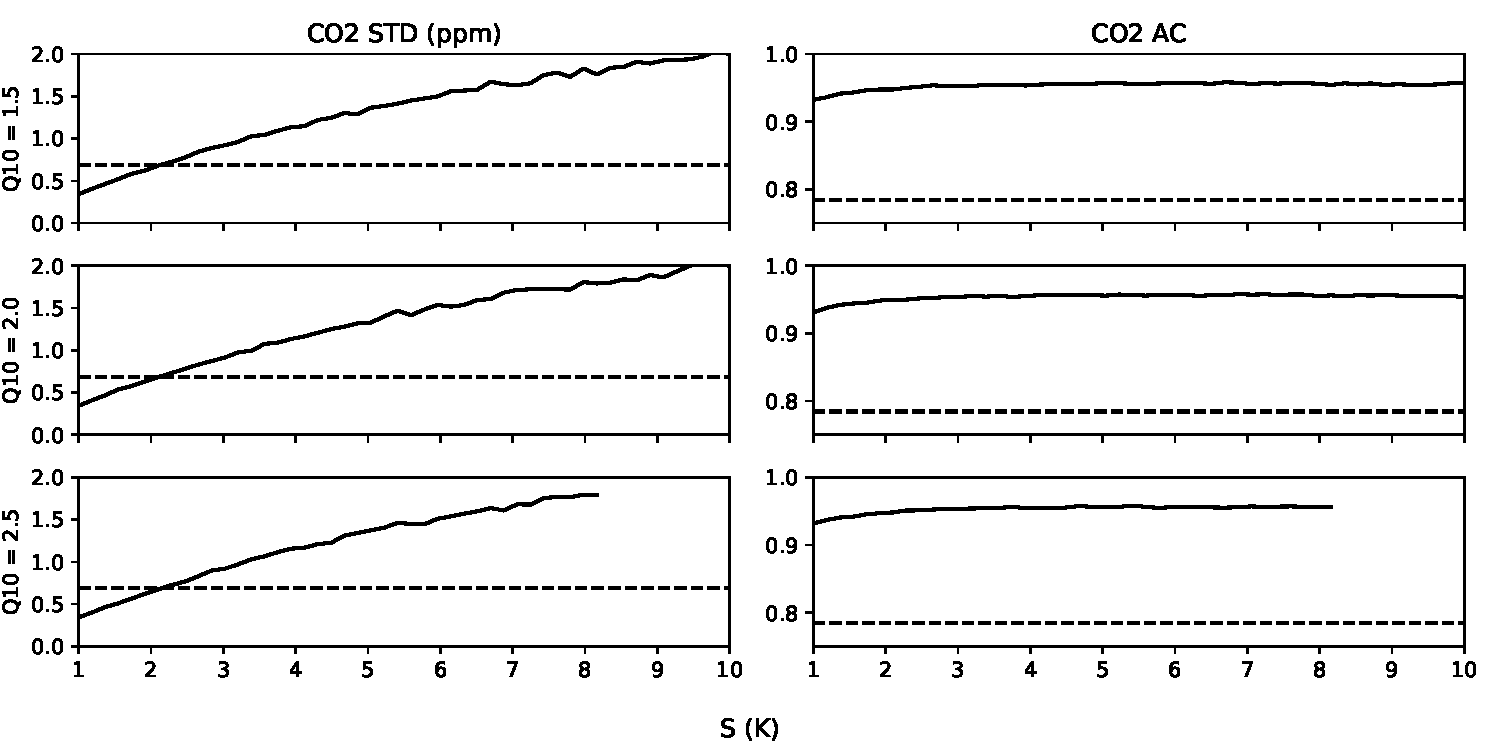
\includegraphics[width=\textwidth]{co2_std_ac}
  \caption[Atmospheric Carbon Variability]{Standard Deviation and Autocorrelation of atmospheric carbon}
  \label{fig:co2_std_ac}
  \end{figure}\todo{do this instead with more complex model}
  \begin{figure}
  \centering
  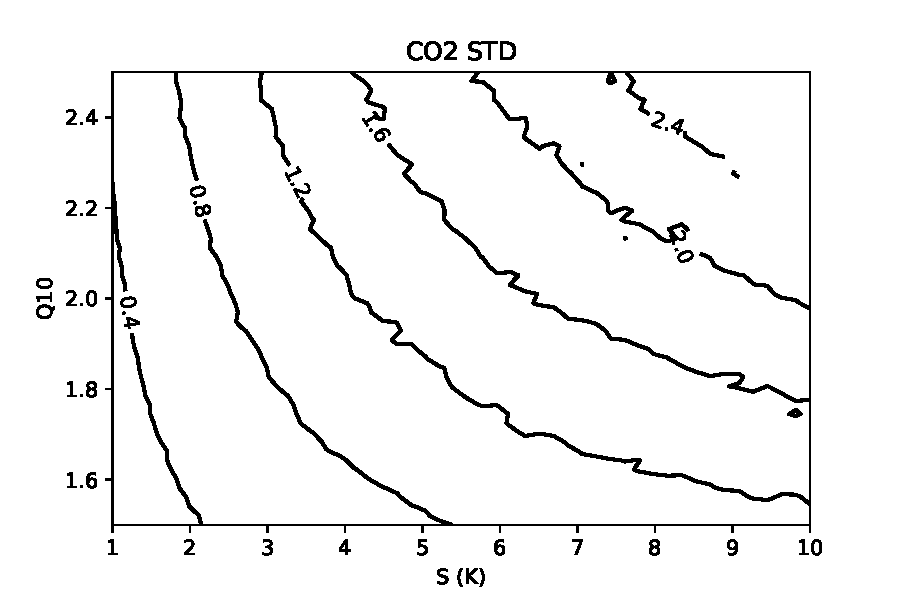
\includegraphics{co2stdcontour}
  \caption{CO2 standard deviation}
  \label{fig:co2_std_Q10_S}
\end{figure}
\begin{figure}
  \centering
  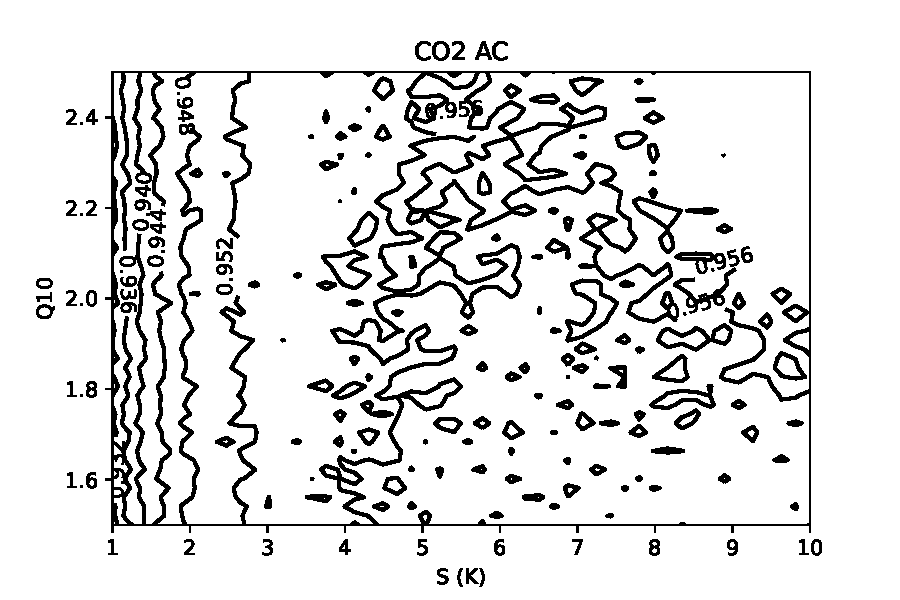
\includegraphics{co2accontour}
  \caption{CO2 AC}
  \label{fig:co2_ac_Q10_S}
\end{figure}